\begin{flalign*}
	&(1)\begin{cases}
		\tilde q = \tilde q(q, t, \alpha) \\
		\tilde t = \tilde t(q, t, \alpha) \\
	\end{cases}
	\qquad
	\det\pd{(\tilde q_1, \ldots, \tilde q_n, \tilde t)}{(q_1, \ldots, q_n, t)} \neq 0
	&\\
	& \tilde q(q, t, 0) = q,\; \tilde t(q, t, 0) = t,\ \tilde L(\tilde q, \tilde q', \tilde t) = L(\tilde q, \tilde q', \tilde t) &\\
	& f = (\eta \cdot p) - \zeta H = const &\\
	& p = \pd{L}{\dot q},\; \eta = \left.\pd{\tilde q}{\alpha}\right|_{\alpha = 0},\; H = \left( \pd{L}{\dot q},\; \dot q \right) - L,\; \zeta = \left.\pd{\tilde t}{\alpha}\right|_{\alpha = 0} &\\
\end{flalign*}
\begin{proof}
\begin{flalign*}
	& (1) \Rightarrow \begin{cases}
		\tilde q = q + \alpha \eta + O_2(\alpha) \\
		\tilde t = t + \alpha \zeta + O_2(\alpha) \\
	\end{cases} (1') &\\
	& \begin{cases}
		q = \tilde q - \alpha \eta + O_2(\alpha) \\
		t = \tilde t - \alpha \zeta + O_2(\alpha) \\
	\end{cases} &\\
	& \dot q = \frac{dq}{dt} = \frac{d}{dt}(\tilde q - \alpha \eta + O_2(\alpha)) = \frac{d\tilde q}{d\tilde t}\frac{d\tilde t}{dt} - \alpha \dot\eta + O_2(\alpha) = q'(1 + \alpha \dot \zeta) - \alpha \dot \eta + O_2(\alpha) &\\
	& \dot q = \tilde q' + \alpha(\dot \zeta \tilde q' - \dot \eta) + O_2(\alpha) = \tilde q' + \alpha(\zeta \dot q - \dot \eta) + O_2(\alpha) \quad (2) &\\
	& \tilde L(\tilde q, \tilde q', \tilde t) = L(q, \dot q, t)|_{(1'),(2)} \cdot \frac{d t}{d \tilde t} = L(\tilde q - \alpha \eta + O_2,\; \tilde q' + \alpha(\zeta\dot q - \dot \eta) + O_2,\; \tilde t - \alpha \zeta + O_2)\cdot \frac{dt}{d \tilde t} = &\\
	& = \left( L(\tilde q, \tilde q', \tilde t) + \alpha \left[ \left( \pd{L}{q}, -\eta \right) + \left( \pd{L}{\dot q}, \zeta \dot q - \dot \eta \right) + \pd{L}{t}(-\zeta)\right] + O_2\right)(1 - \alpha\dot \zeta + O_2) = &\\
	& = L(\tilde q, \tilde q', \tilde t) + \alpha\left[ -\left( \frac{d}{dt}\pd{L}{\dot q}, \eta \right) - \left( \pd{L}{\dot q}, \dot \eta \right) + \dot \zeta\left( \pd{L}{\dot q}, \dot q \right) - \dot \zeta L - \pd{L}{t}\zeta\right] + O_2 = &\\
	& = L(\tilde q ,\tilde q', \tilde t) + \alpha\left[ -(\dot p, \eta) - (p, \dot \eta) + \dot \zeta H + \pd{H}{t} \zeta\right] + O_2 = &\\
	& L(\tilde q, \tilde q', \tilde t) - \alpha \frac{d}{dt}f + O_2(\alpha) = L(\tilde q, \tilde q', \tilde t) &\\
	& \left.\frac{d}{d\alpha}\right|_{\alpha = 0} \Leftrightarrow \frac{df}{dt} = 0 \Leftrightarrow f = const &\\
\end{flalign*}
\end{proof}

\subsection{Интегральный инвариант}
\begin{figure}[H]
	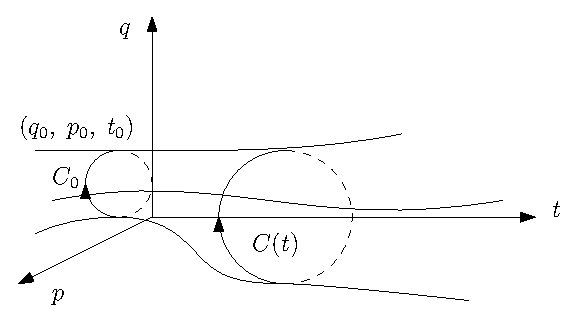
\includegraphics{9_1.eps}
\end{figure}
\begin{flalign*}
	& H = H(q, p, t) &\\
	& (*) \begin{cases}
	\dot q = \pd{H}{p} \\
	\dot p = -\pd{H}{q} \\
	\end{cases} &\\
	& \{q, p, t\} \text{ --- расширенное фазовое пространство.} &\\
	& \begin{cases}
	q = q(t,\; q_0,\; p_0) \\
	p = p(t,\; q_0,\; p_0) \\
	\end{cases}
	\text{ --- прямой путь.} &\\
	& C_0 \rightarrow C(t) &\\
	& I_{\text{п}} = \oint\limits_{C: t = const} \sum\limits_{i = 1}^np_i \delta q_i = \oint(p,\delta q) \text{ --- универсальный интегральный инвариант Пуанкаре.} &\\
\end{flalign*}
\begin{ass}
	Величина $I_{\text{п}}$ сохраняется на всех контурах (изохронах), охватывающих одну и ту же трубку прямых путей системы $(*)$.
\end{ass}
\begin{proof}
	\begin{flalign*}
		& C(t): \begin{cases}
		q = q(\alpha), &\alpha \in [0; 1] \\
		p = p(\alpha), &q(0) = q(1) \\
		t = const, &p(0) = p(1) \\
		\end{cases} &\\
		& \delta q = \pd{q}{\alpha}\delta \alpha &\\
		& \frac{d}{dt} I_{\text{п}} = \oint\limits_C (\dot p, \delta q) + (p, \dot{(\delta q)}) \ovalbox{=} &\\
		& \frac{d}{dt}\delta q = \frac{d}{dt}\left( \pd{q}{\alpha} \right)\delta \alpha = \pdd{\frac{d}{dt}q}{\alpha}\delta \alpha = \delta \dot q &\\ 
		& \ovalbox{=} \oint\limits_C (\dot q, \delta q) + (p, \delta \dot q) = \oint\limits_C \delta(p, \dot q) - \oint\limits_C(\delta p, \dot q) + \oint\limits_C (\dot p, \delta q) \overset{(*)}{=} &\\
		& \overset{(*)}{=} -\oint\limits_C\left( \pd{H}{p}, \delta p \right) + \left( \pd{H}{q}, \delta q \right) = -\oint\limits_C \delta H = 0 \Rightarrow I_{\text{п}} = const
	\end{flalign*}
\end{proof}

\begin{df}
	\[
		I = \oint\big[(A(q,\; p,\; t),\delta q) + (B(q,\; p, \; t), \delta p) + \gamma(q,\; p, \; t)\delta t\big]
	\]
	$I$ --- относительный интегральный инвариант первого порядка системы $(*)$, если $I$ сохраняет свое значение на всех согласованных контурах, охватывающих одну и ту же трубку прямых путей.
\end{df}
\begin{df}
	Контуры согласованы, если если существует такая их параметризация, что каждому значению параметра разных контуров соответствуют точки одного и того же пути.
\end{df}
\begin{figure}[H]
	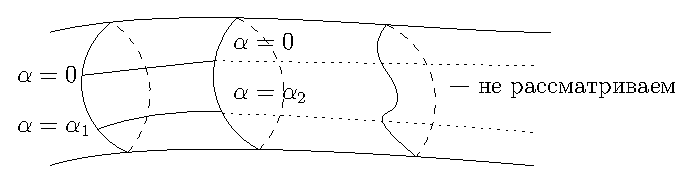
\includegraphics{9_2.eps}
\end{figure}

\begin{teo}[Теорема Ли Хуа-Чжуна]
	\[ 
		I = \oint\limits_{C: t = const} (A(q,\; p,\; t), \delta q) + (B(q,\; p, \; t), \delta p)
	\] 
	--- универсальный (не зависит от гамильтониана) интегральный инвариант системы $(*)$ тогда, и только тогда, когда $I = cI_\text{п},\; c = const$
\end{teo}
\begin{proof}
Для простоты $n = 1$.
\begin{flalign*}
	& \frac{d}{dt} I = \frac{d}{dt} \oint\limits_{C: t = const} A\delta q + B \delta q = \oint\limits_C \dot A\delta q + \dot B \delta p + A\delta \dot q + B \delta\dot p =  \oint\limits_C \delta(A\dot q + B \dot p) - \delta A\dot q - \delta B \dot p + \dot A\delta q + \dot B\delta p = &\\
	& = \oint\limits_C \left( \pd{A}{p}\dot p + \cancel{\pd{A}{q}\dot q} + \pd{A}{t} \right)\delta q - \left( \pd{A}{p} \delta p  + \cancel{\pd{A}{q}\delta q}\right)\dot q + \left(\cancel{\pd{B}{p}\dot p} + \pd{B}{q}\dot q + \pd{B}{t} \right)\delta p - \left( \cancel{\pd{B}{p}\delta p} + \pd{A}{q}\delta q \right)\dot p = &\\
	& = \oint\limits_C -\left( \pd{A}{p} - \pd{B}{q} \right)\pd{H}{p}\delta p + \left( \pd{A}{p} - \pd{B}{q} \right)\left( -\pd{A}{q} \right)\delta q + \pd{A}{t}\delta q + \pd{B}{t}\delta p = &\\
	& = \oint\limits_C \underbrace{\alpha\delta p + \beta\delta q}_{\delta f} = 0 \quad \forall C \Leftrightarrow \pd{f}{q} &\\
	& \begin{cases}
		\pd{f}{q} = -z\pd{H}{q} + \pd{A}{t},\; z = \pd{A}{t} - \pd{B}{q} \\
		\pd{f}{q} = -z \pd{H}{p} + \pd{B}{t} \\
	\end{cases} &\\
	& \frac{\partial^2f}{\partial q \partial p} = \frac{\partial^2 f}{\partial p \partial q} \Leftrightarrow -\pd{z}{p}\pd{H}{q} - \cancel{z\frac{\partial^2H}{\partial p\partial q}} + \frac{\partial^2 A}{\partial p\partial t} = -\pd{z}{p}\pd{H}{q} - \cancel{z\frac{\partial^2H}{\partial q \partial p}} + \frac{\partial^2 B}{\partial q \partial t} &\\
	& -\pd{z}{p}\pd{H}{q} + \pd{z}{q}\pd{H}{p} + \pd{z}{t} = 0 \; \forall H \Leftrightarrow \pd{z}{p} = \pd{z}{q} = \pd{z}{t} = 0 \Leftrightarrow z = c = const &\\
	& \pd{A}{p} - \pd{B}{q} = c &\\
	& \pdd{A - cp}{p} = \pd{B}{q} \Leftrightarrow (A - cp)\delta q + B\delta p = 0 &\\
	& A\delta p + B\delta p = cp\delta q \Rightarrow I = cI_\text{п} &\\
\end{flalign*}
\end{proof}
\begin{df}
	$ I_\text{пк} = \oint (p, d q) - Hd t $ --- интегральный инвариант Пуанкаре-Картана.
\end{df}
\begin{ass}
	$I_\text{пк} = const$.
\end{ass}
\begin{proof}
\begin{figure}[H]
	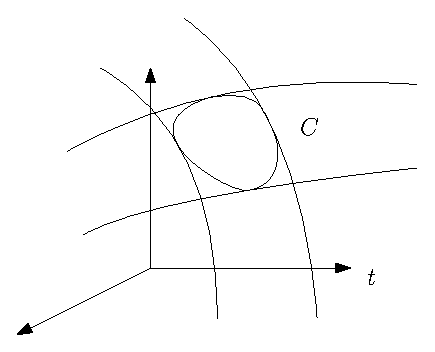
\includegraphics{9_3.eps}
\end{figure}
\begin{flalign*}
	& C:\tau(q, p, t) = const &\\
	& q_{n + 1} = t &\\
	&\begin{cases}
	\dot q = \pd{H}{p} \\
	\dot p = -\pd{H}{q} \\
	\end{cases} &\\
	& q' = \frac{dq}{d\tau} = \frac{dq}{dt}\frac{dt}{d\tau} = \frac{dH}{dp}\eta &\\
	& \eta(q,\; p,\; q_{n + 1}) = \pd{t}{\tau} &\\
	& p' = \frac{dp}{d\tau} = -\pd{H}{q}\eta &\\
	& p_{n + 1} = -H(q,\; p,\; t) \quad q_{n + 1}' = \frac{dt}{d\tau}= \eta &\\
	& \tilde H = \eta(H + p_{n + 1}) \qquad p_{n + 1}' = -\pd{H}{q_{n + 1}}\eta = -\pd{H}{t}\eta &\\
	& \text{Докажем, что $\tilde H$ --- новый гамильтониан.} &\\
	& \pd{\tilde H}{p} = \pd{\eta}{p}(H + p_{n + 1}) + \eta \pd{H}{p} = \eta \pd{H}{p} = q' &\\
	& \pd{\tilde H}{q} = \pd{\eta}{q}(H + p_{n + 1}) + \eta\pd{H}{q} = \eta \pd{H}{q} = - p' &\\
	& \pd{H}{p_{n + 1}} = \eta = q_{n + 1}',\; \pd{\tilde H}{q_{n + 1}} = \pd{\eta}{q_{n + 1}}(H + p_{n + 1}) + \eta\pd{H}{q_{n + 1}} = \frac{dt}{d\tau}\pd{H}{t} = -p_{n + 1}' &\\
	& I = \oint\limits_C(\tilde p, \delta \tilde q) \text{ --- инвариант } \Rightarrow I_\text{пк} = \oint(p, dq) - Hdt &\\
\end{flalign*}
\end{proof}
\begin{flalign*}
	& I = \int\ldots\int dq_1 \ldots dq_n dp_1 \ldots dp_n = V &\\ 
\end{flalign*}